\hypertarget{heat2D_8cpp}{
\subsection{/home/luiggi/Documents/Research/Meshless\_\-RBF/NEW/RBFSoft/examples/02Heat2D/heat2D.cpp File Reference}
\label{heat2D_8cpp}\index{/home/luiggi/Documents/Research/Meshless\_\-RBF/NEW/RBFSoft/examples/02Heat2D/heat2D.cpp@{/home/luiggi/Documents/Research/Meshless\_\-RBF/NEW/RBFSoft/examples/02Heat2D/heat2D.cpp}}
}
Poisson equation in 2D.  




\subsubsection{Detailed Description}
Poisson equation in 2D. 

The PDE to solve is: \[ \frac{\partial^2 T}{\partial x^2}+\frac{\partial^2 T}{\partial y^2}=0 \] and the boundary conditions are as shown in the next figure:  \begin{Image}
\begin{center}
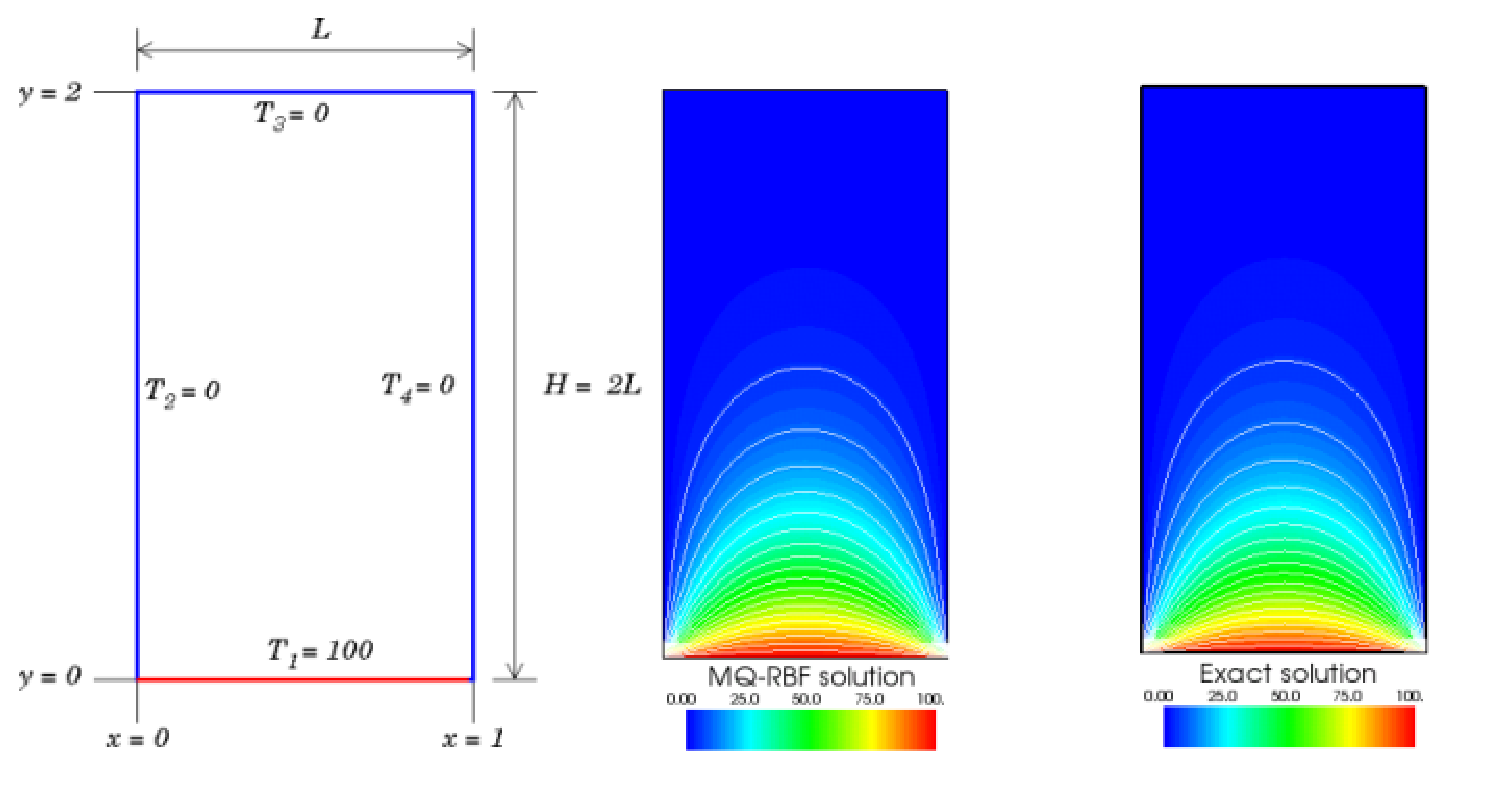
\includegraphics[width=5cm]{solHoffman}\caption{Geometry, boundary conditions and solution}
\end{center}
\end{Image}
 \begin{Desc}
\item[Input]The {\tt input} file contains the following initial data:\begin{itemize}
\item {\tt hx}, {\tt hy}, {\tt Nx}, {\tt Ny} : Lenghts of the rectangle, and number of points in each axis.\item {\tt rtype}, {\tt ep}, {\tt layer} : Type of knots distribution, randomness, layer around the domain.\item {\tt c} : Shape parameter for MQ-RBF kernel ($c < 0$ implies $ c = 1/\sqrt{N}$).\item {\tt fsol} : choose a method to solve the system.\item {\tt max\_\-knots} : neighbors used to construct the ACBF preconditioner. \end{itemize}
\end{Desc}
\begin{Desc}
\item[Output]\begin{itemize}
\item {\tt xy\_\-knots.dat} (x,y) coordinates of random points;\item {\tt solution.dat} (x,y,u) evaluation of the solution in a grid;\item {\tt errordis.dat} (x,y,e) error distribution in a grid;\item {\tt exactsol.dat} (x,y,u) exact solution in a grid;\end{itemize}
\end{Desc}
\begin{Desc}
\item[Author:]Luis M. de la Cruz \mbox{[} Thu Sep 6 14:35:41 BST 2007 \mbox{]} \end{Desc}


Definition in file \hyperlink{heat2D_8cpp-source}{heat2D.cpp}.